\message{ !name(billets.tex)}\documentclass[11pt]{book}
\usepackage[a4paper, total={20cm, 28cm}]{geometry}
\usepackage{palatino}
\usepackage{tikz}
\usetikzlibrary{calc} 


\begin{document}

\message{ !name(billets.tex) !offset(-3) }

\foreach \n in {1,...,100} {

  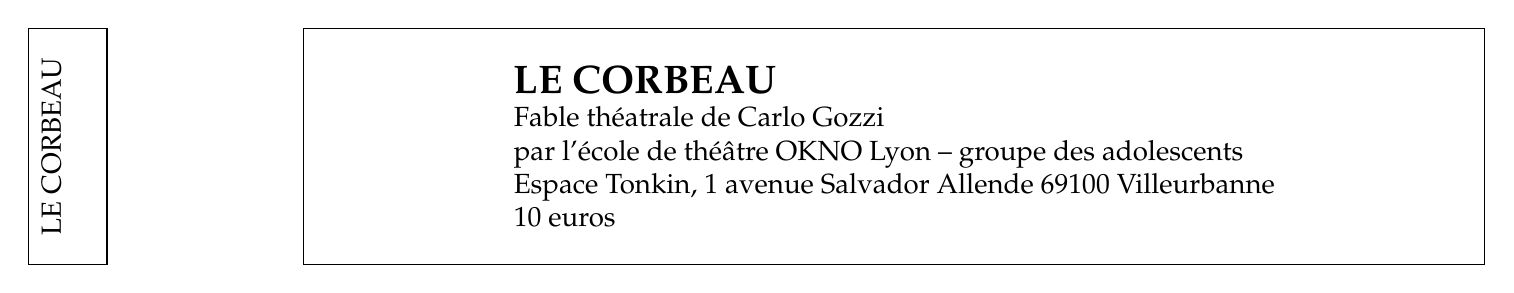
\begin{tikzpicture}
    \draw(0,0) rectangle ++(1,3) node[midway, align=center, rotate=90] {LE CORBEAU\\\textbf{\n}};
    \draw(3.5,0) rectangle ++(15,3) node[midway, align=left]
    {{\Large \textbf{LE CORBEAU}}\\
      Fable théatrale de Carlo Gozzi\\
      par l'école de théâtre OKNO Lyon -- groupe des adolescents\\
      Espace Tonkin, 1 avenue Salvador Allende 69100 Villeurbanne\\
      10 euros
    }
    node[below left]{\Large \textbf{\n}};
  \end{tikzpicture}
  ~\\
}
\end{document}

\message{ !name(billets.tex) !offset(-29) }
